
\section{SATD削除期間や割合についての調査\cite{satd-removal}}

\subsection{概要}
近年では,コードからSATDを検出する手法の開発や,ソフトウェア品質への影響を調査する研究が実施されている.しかし,SATDはプロジェクト内に10年以上存在する場合もあり,これは全てのSATDが「悪い」とされているわけではなく,削除すべきSATDもあれば,削除しなくても問題ないSATDがあることも示している.
そこで文献\cite{satd-removal}では,SATDの削除に焦点を当てた研究を行っている.5つのオープンソースプロジェクトのJavaファイルについて,以下の4つのRQに基づいて調査を行っている.

\begin{itemize}
  \item RQ 1: どの程度のSATDが削除されているのか?
  \item RQ 2: 誰がSATDを削除しているのか?
  \item RQ 3: SATDはどれくらいの期間,プロジェクト内に存続するのか?
  \item RQ 4: SATDの削除はどのような活動によって行われるのか?
\end{itemize}

% ====== 結果いるのかな? ==========
% その結果,SATDの大部分は削除されており,大部分がSATDを導入した本人により削除されていたということが明らかになっている.さらに,SATDは中央値で約18日~約170日の期間で持続し,開発者はバグの修正や新機能の追加の際に,SATDを削除することが多いということが明らかになっている.

\subsection{データの前処理}
ここでは,文献\cite{satd-removal}で用いられてるデータとその事前処理について説明する.文献\cite{satd-removal}では,より多くの数・種類のSATDについて,その変化を調査するために,コメント数が多く,活動性が高いプロジェクトに焦点を当てている.選定された5つのオープンソースプロジェクト(Camel、Gerrit、Hadoop、Log4j、Tomcat)は,Javaを用いてGit上で開発されている.

\begin{figure}[t]
    \centering
    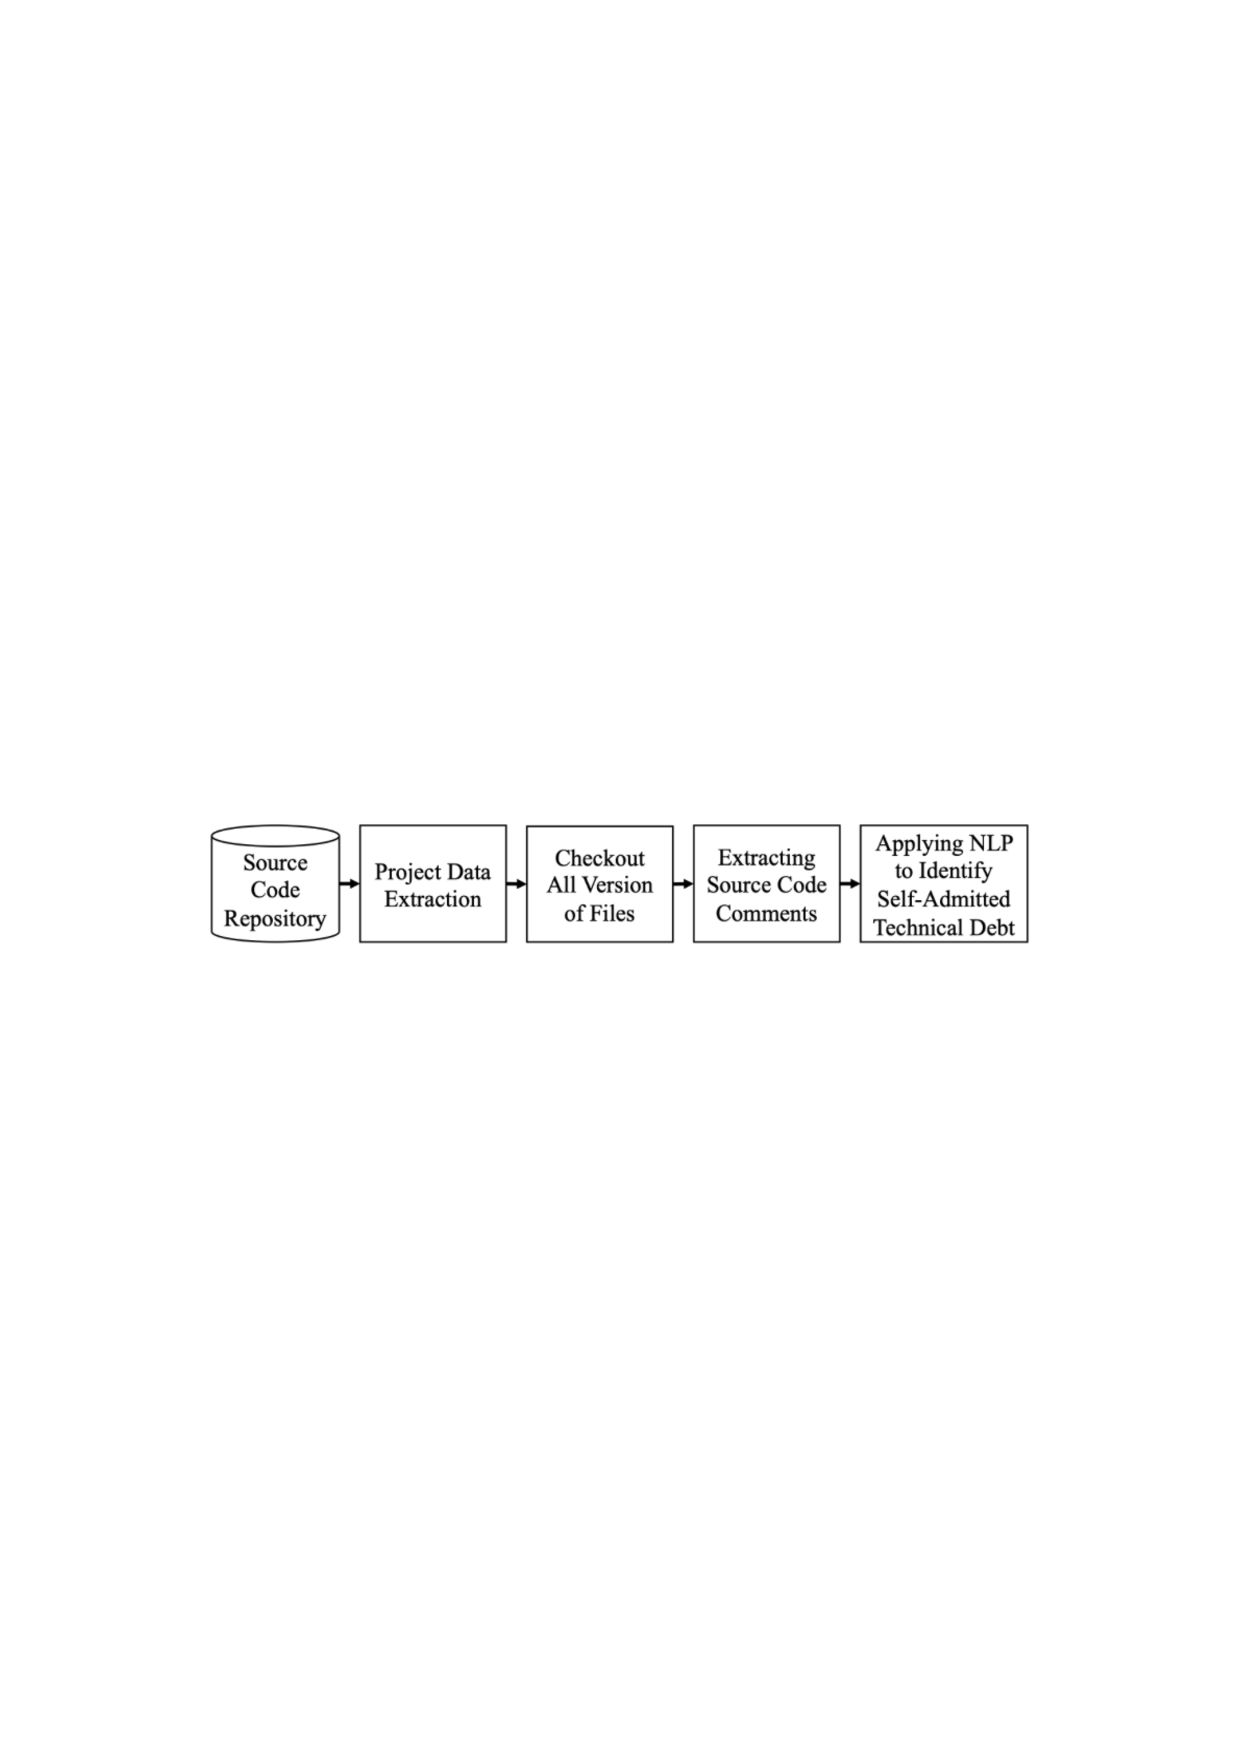
\includegraphics[width=0.9\linewidth, angle=0]{./thesis1/data-preprocess1.pdf}
    \caption{データ処理工程}
    \label{fig:1_data-preprocess}
\end{figure}

図\ref{fig:1_data-preprocess}にデータ処理の工程を示す.ExtracttingSourceCodeCommentでは,明らかに負債ではないライセンスコメントやIDEによる自動生成コメントを削除している.Applying NLP ではSATDのコメントを特定するために,Maldonadoら\cite{1-ref-25}の手法を用いている.NLP分類器は\cite{1-ref-25}によって提供されたデータを用いて訓練されたものを使用している.

各工程後に取得したデータの詳細を表\ref{fig:1_data-table},表\ref{fig:1_data-satd-table}に示す.

\begin{table*}[t]
    \centering
    \caption{調査対象プロジェクトの詳細}
    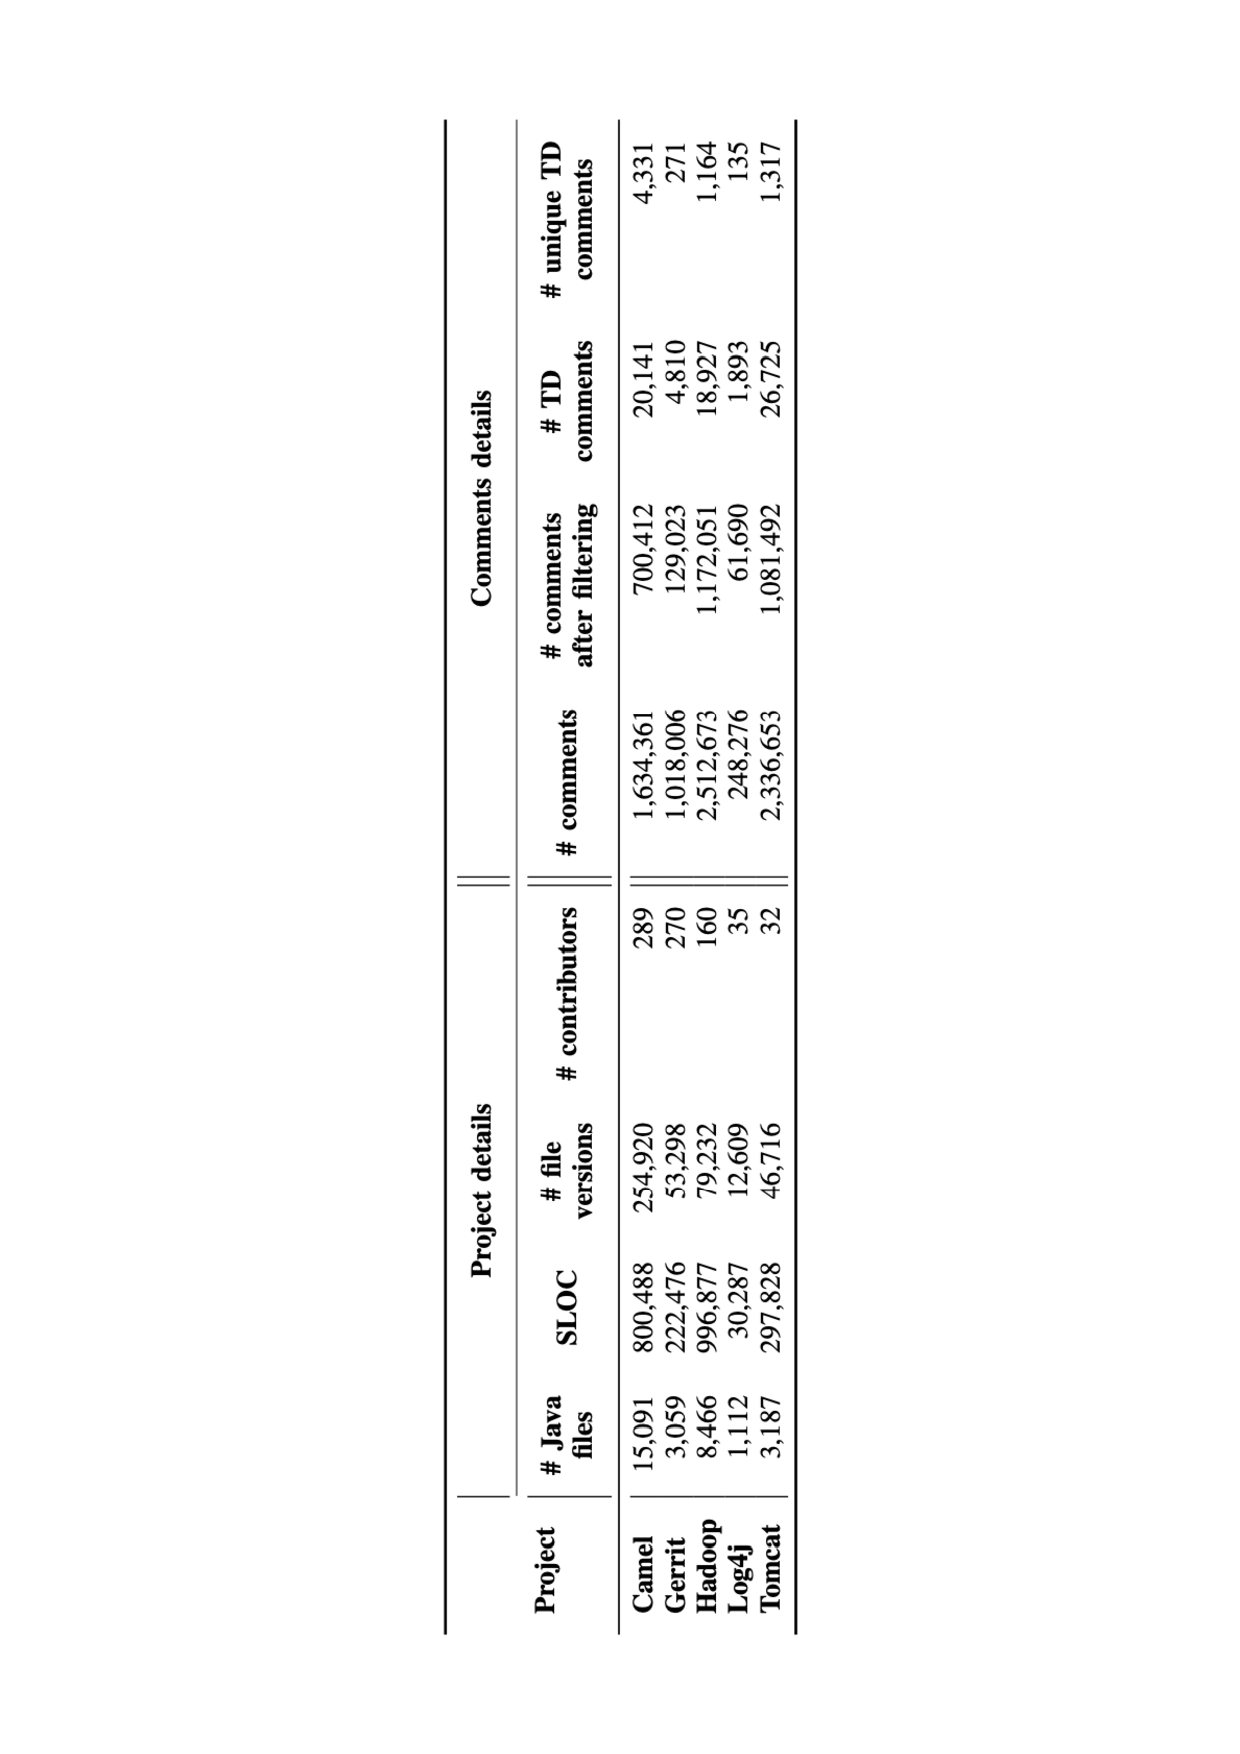
\includegraphics[height=0.9\linewidth, angle=270]{./thesis1/data-table1.pdf}
    \label{fig:1_data-table}
\end{table*}


% 全てのファイルのバージョンの特定後に,コメントを削除したコミットの日付を削除日とみなしている.また,ファイルがリネームされたり,別のフォルダに移動された場合で,古いバージョンと少なくとも90\%以上が類似している場合に,Gitはそのファイルが移動またはリネームされたファイルとして判断している.

% 技術的負債に焦点を当てるために事前に,明らかに負債ではない以下のタイプのコメントを除外する.それにより,Camelプロジェクトではコメント数を,1,634,361件から700,412件に減らしている.

% \begin{itemize}
%   \item ライセンスコメント
%   \item コメントアウトされたソースコード
%   \item IDE による自動生成コメント
%   \item Javadoc のコメント
% \end{itemize}

% SATDのコメントを特定するために,Maldonadoら\cite{1-ref-25}の手法用いている.\cite{1-ref-25}によって提供されたデータを用いて訓練されたNLP分類器を適用した結果を表\ref{fig:1_data-satd-table}に示す.


\begin{table}[t]
    \centering
    \caption{調査対象プロジェクト内SATDの詳細}
    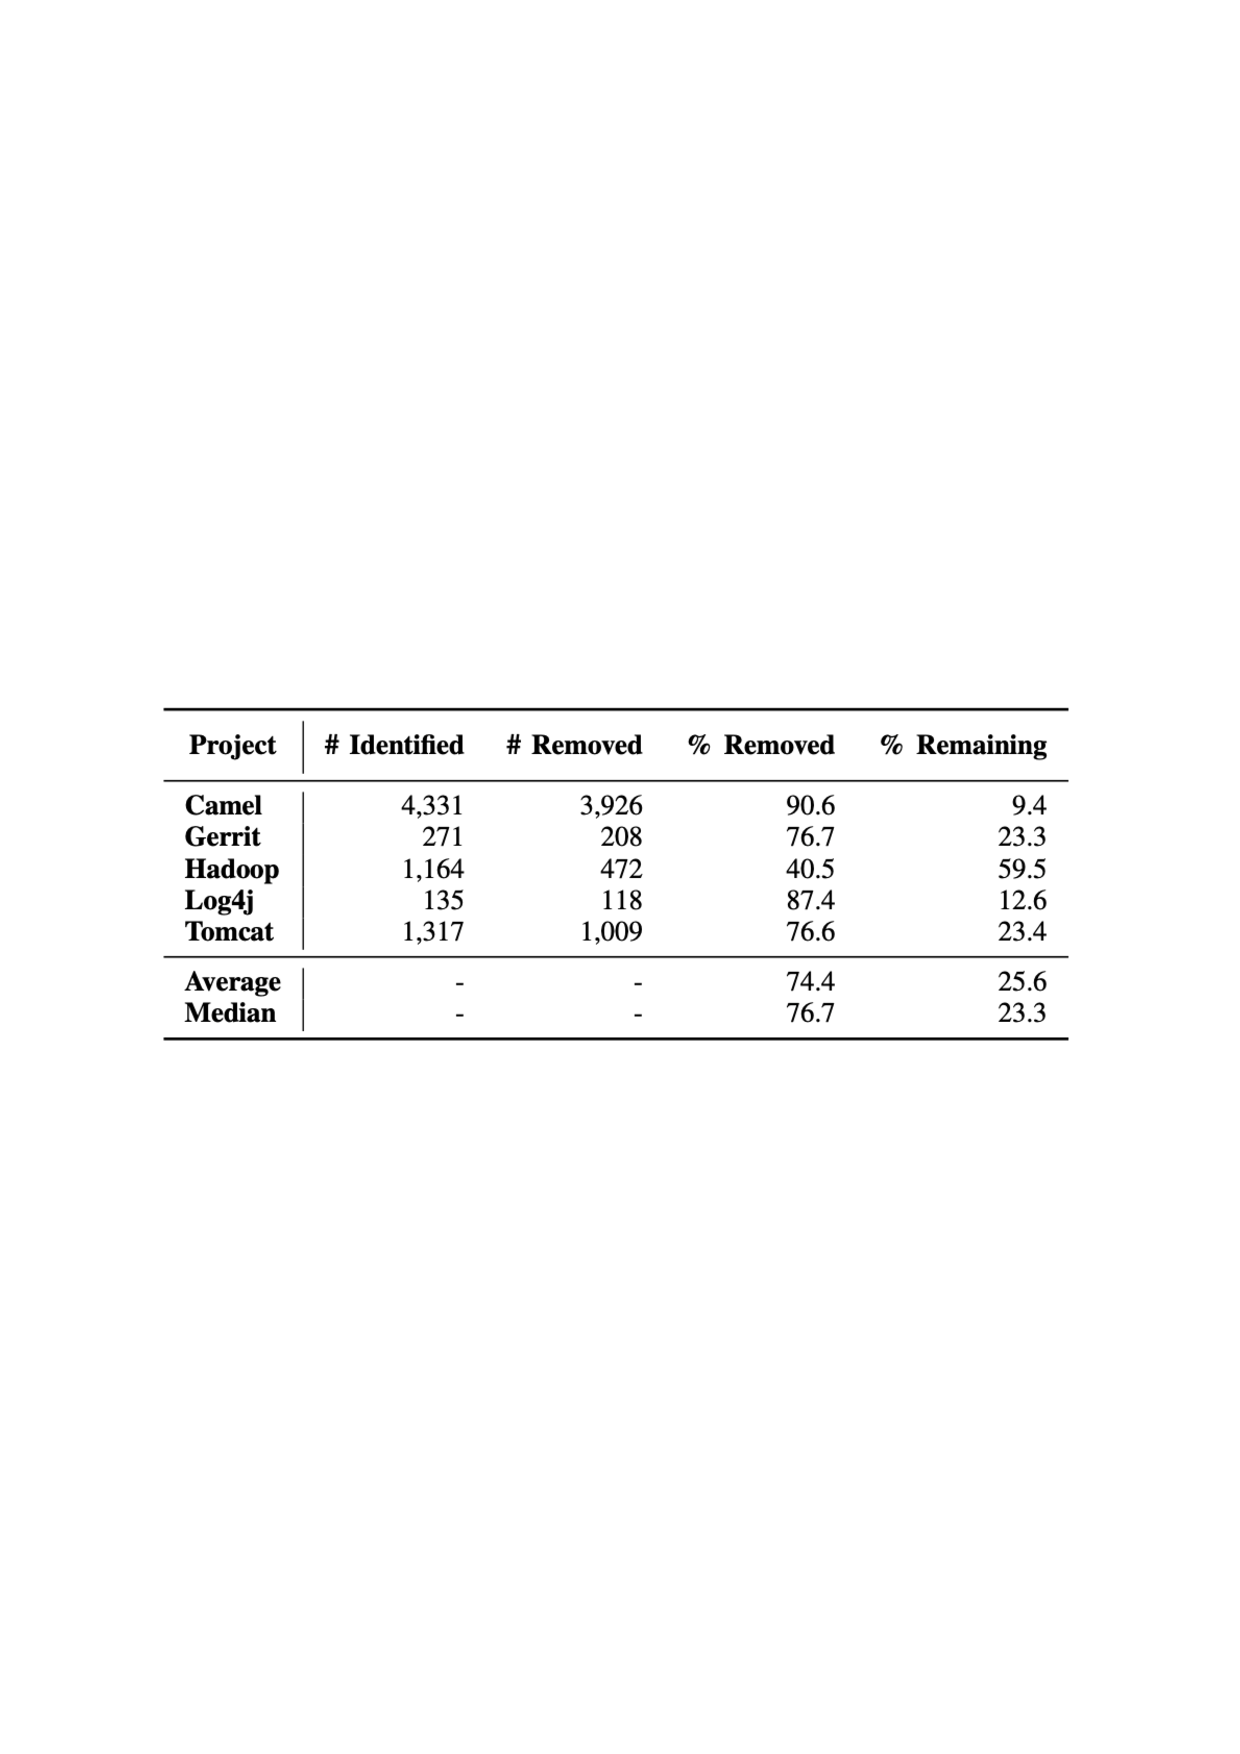
\includegraphics[width=0.9\linewidth, angle=0]{./thesis1/data-satd-table1.pdf}
    \label{fig:1_data-satd-table}
\end{table}



\subsection{結果}
以前の研究では,SATDの検出,管理,影響について検討されてきたが,そのようなSATDの削除については,ほとんど知られていなかった.文献\cite{satd-removal}では,SATDの削除について調査を行なっており,
その結果,SATDの大部分は削除され(平均74.4%),また大部分はSATDを導入した本人により削除され(平均54.4%),削除されるまでの期間は平均82~613.2日であることがわかっている.
さらに14名の開発者を対象に,SATDの導入と削除の理由について調査を実施している.調査の結果,開発者はSATDを削除する必要性を認識しているにもかかわらず,SATDを削除するための正式なプロセスはなく,ほとんどの削除はバグ修正の一環として行われていることを発見している.したがって,文献\cite{satd-removal}では,プロジェクトが効果的かつ体系的にSATDに対処できるような技術が必要であるということが示唆されている.



% ====== RQについてそれぞれで結果を書くと長くなるため削除しました ========
% \subsection{結果}
% ここでは\cite{satd-removal}のRQ1~RQ4についての結果を紹介する.

% \subsubsection{RQ1}

% 表\ref{fig:1_data-satd-table}プロジェクトごとの削除されたSATDコメントを示す.表\ref{fig:1_data-satd-table}よりSATDコメントの大部分(平均74.4\%,中央値76.7\%)が削除されていることがわかり,開発者がSATDを認識し,意識しているという傾向が示されている.

% \subsubsection{RQ2}
% 調査結果によると,ほとんどの場合SATDの大部分が,それを導入したのと同じ著者によって削除されている.平均すると,全SATD除去の54.4\%が導入した本人による削除であり,対象にした5つのプロジェクトのうち4つのプロジェクトでは自己除去が50\%以上を占めている.

% \subsubsection{RQ3}
% 一般的に,SATDがプロジェクトに留まる時間はプロジェクトによって異なり,中央値は18.2~172.8日,平均値は82~613.2日である.すべてのプロジェクトにおいて,最初の数百日でSATDは削除されており,クリティカルなSATDは急速に削除されるということが示されているが,プロジェクトにより急速に削除される期間や削除が緩やかになる期間に差がある.また,RQ2のデータをもとに,自己削除したSATDとそうでないSATDを比較し,自己削除したSATDの方が早く削除されるという結果も発見されている.


